% comment out for student version
\ifdefined\Student\relax\else\def\Teacher{}\fi

\documentclass[12pt]{article}

\title{Activity 11: Designing Classes}
\author{Chris Mayfield and Helen Hu}
\date{Fall 2018}

%\ProvidesPackage{cspogil}

% fonts
\usepackage[utf8]{inputenc}
\usepackage[T1]{fontenc}
\usepackage{mathpazo}

% spacing
\usepackage[margin=2cm]{geometry}
\renewcommand{\arraystretch}{1.4}
\setlength{\parindent}{0pt}

% orphans and widows
\clubpenalty=10000
\widowpenalty=10000
\pagestyle{empty}

% figures and tables
\usepackage{graphicx}
\usepackage{multicol}
\usepackage{tabularx}
\usepackage{wrapfig}

% fixed-width columns
\usepackage{array}
\newcolumntype{L}[1]{>{\raggedright\let\newline\\\arraybackslash\hspace{0pt}}m{#1}}
\newcolumntype{C}[1]{>{\centering\let\newline\\\arraybackslash\hspace{0pt}}m{#1}}
\newcolumntype{R}[1]{>{\raggedleft\let\newline\\\arraybackslash\hspace{0pt}}m{#1}}

% include paths
\makeatletter
\def\input@path{{Models/}{../../Models/}}
\graphicspath{{Models/}{../../Models/}}
\makeatother

% colors
\usepackage[svgnames,table]{xcolor}
\definecolor{bgcolor}{HTML}{FAFAFA}
\definecolor{comment}{HTML}{007C00}
\definecolor{keyword}{HTML}{0000FF}
\definecolor{strings}{HTML}{B20000}

% table headers
\newcommand{\tr}{\bf\cellcolor{Yellow!10}}

% syntax highlighting
\usepackage{textcomp}
\usepackage{listings}
\lstset{
    basicstyle=\ttfamily\color{black},
    backgroundcolor=\color{bgcolor},
    numberstyle=\scriptsize\color{comment},
    commentstyle=\color{comment},
    keywordstyle=\color{keyword},
    stringstyle=\color{strings},
    columns=fullflexible,
    keepspaces=true,
    showlines=true,
    showstringspaces=false,
    upquote=true
}

% code environments
\newcommand{\java}[1]{\lstinline[language=java]{#1}}%[
\lstnewenvironment{javalst}{\lstset{language=java,backgroundcolor=}}{}
\lstnewenvironment{javabox}{\lstset{language=java,frame=single,numbers=left}\quote}{\endquote}

% PDF properties
\usepackage[pdftex]{hyperref}
\urlstyle{same}
\makeatletter
\hypersetup{
  pdftitle={\@title},
  pdfauthor={\@author},
  pdfsubject={\@date},
  pdfkeywords={},
  bookmarksopen=false,
  colorlinks=true,
  citecolor=black,
  filecolor=black,
  linkcolor=black,
  urlcolor=blue
}
\makeatother

% titles
\makeatletter
\renewcommand{\maketitle}{\begin{center}\LARGE\@title\end{center}}
\makeatother

% boxes [optional height]
\newcommand{\emptybox}[1][10em]{
\vspace{1em}
\begin{tabularx}{\linewidth}{|X|}
\hline\\[#1]\hline
\end{tabularx}}

% models
\newcommand{\model}[1]{\section{#1}\nopagebreak}
\renewcommand{\thesection}{Model~\arabic{section}}

% questions
\newcommand{\quest}[1]{\subsection*{Questions~ (#1)}}
\newcounter{question}
\newcommand{\Q}{\vspace{1em}\refstepcounter{question}\arabic{question}.~ }
\renewcommand{\thequestion}{\#\arabic{question}}

% sub-question lists
\usepackage{enumitem}
\setenumerate[1]{label=\alph*)}
\setlist{itemsep=1em,after=\vspace{1ex}}

% inline answers
\definecolor{answers}{HTML}{C0C0C0}
\newcommand{\ans}[1]{%
\ifdefined\Student
    \leavevmode\phantom{~~\textcolor{answers}{#1}}
\else
    ~~\textcolor{answers}{#1}
\fi}

% longer answers [optional height]
\newsavebox{\ansbox}
\newenvironment{answer}[1][4em]{
\nopagebreak
\begin{lrbox}{\ansbox}
\begin{minipage}[t][#1]{\linewidth}
\color{answers}
}{
\end{minipage}
\end{lrbox}
\ifdefined\Student
    \phantom{\usebox{\ansbox}}%
\else
    \usebox{\ansbox}%
\fi}


\begin{document}

\maketitle

Previously we explored how classes define attributes and methods.
Static variables and methods apply to the whole class, whereas non-static variables and methods apply to specific objects.

\guide{
  \item Discuss benefits of POGIL for student learning.
  \item Explain the purpose of constructor, accessor, and mutator methods.
  \item Implement the equals and toString methods for a given class design.
  \item Design a new class (UML diagram) based on a general description.
}{
  \item Identifying attributes and data types that model a real-world object. (Problem Solving)
}{
\ref{pogil-research.tex} is a meta activity designed to reestablish buy-in near the end of the semester.
Be sure to explain why you are using POGIL in your classroom and how it benefits students.
The figures and sample solutions are from Moog (2014), found in Chapter 8 of \href{http://dx.doi.org/10.7936/K7PN93HC}{Integrating Cognitive Science with Innovative Teaching in STEM Disciplines}.

\ref{common-methods.tex} begins with questions about constructors, getters, and setters.
Report out on \ref{immutable} as soon as the majority teams have made it that far.
Reinforce the concept of immutable objects, and point out that the \java{java.lang.String} class is designed this way.

The questions immediately after \ref{expr} require students to understand the source code of \java{equals} and \java{toString}.
If this is the first time they have seen language features like \java{Object}, \texttt{instanceof}, and \java{String.format}, you may want to give a 5-minute lecture (but avoid giving the answers).

When reporting out \ref{credit-card.tex}, have presenters write their designs on the board.
Compare the trade-offs of their different designs.
For example, to store credit card numbers some teams may use strings, others may use arrays of integers, and some may use a \texttt{long} variable (\texttt{int} won't work because of the range).
}

\section*{Meta Activity: POGIL Research}

\textit{Process-Oriented Guided Inquiry Learning} (see \href{https://pogil.org/}{pogil.org}) is a student-centered, group-learning instructional strategy and philosophy developed through research on how students learn best.
The following two figures are from peer-reviewed articles published in education journals.

% images from Chapter 8 of http://dx.doi.org/10.7936/K7PN93HC

\vspace{1em}
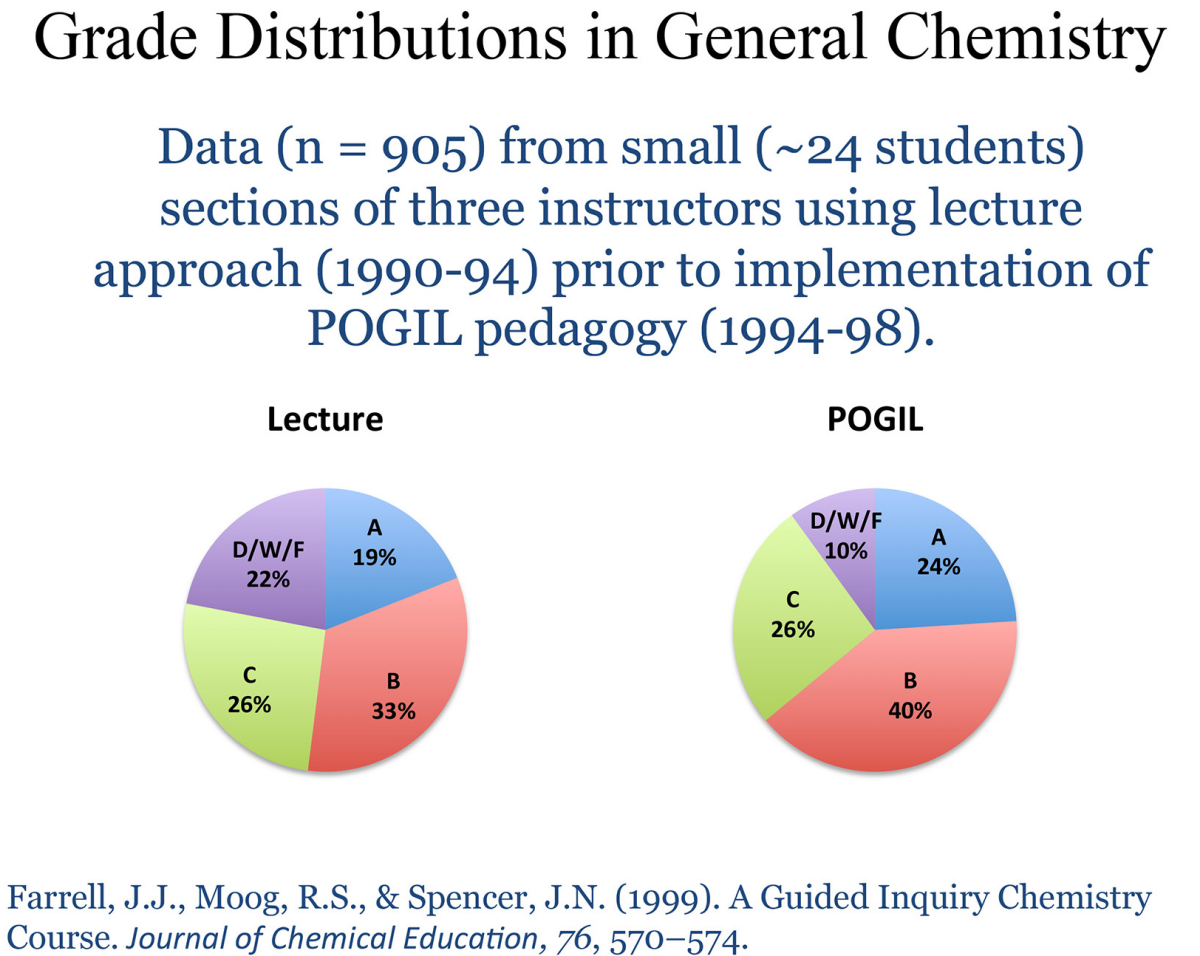
\includegraphics[width=0.47\linewidth]{pogil-grades.png}
\hfill
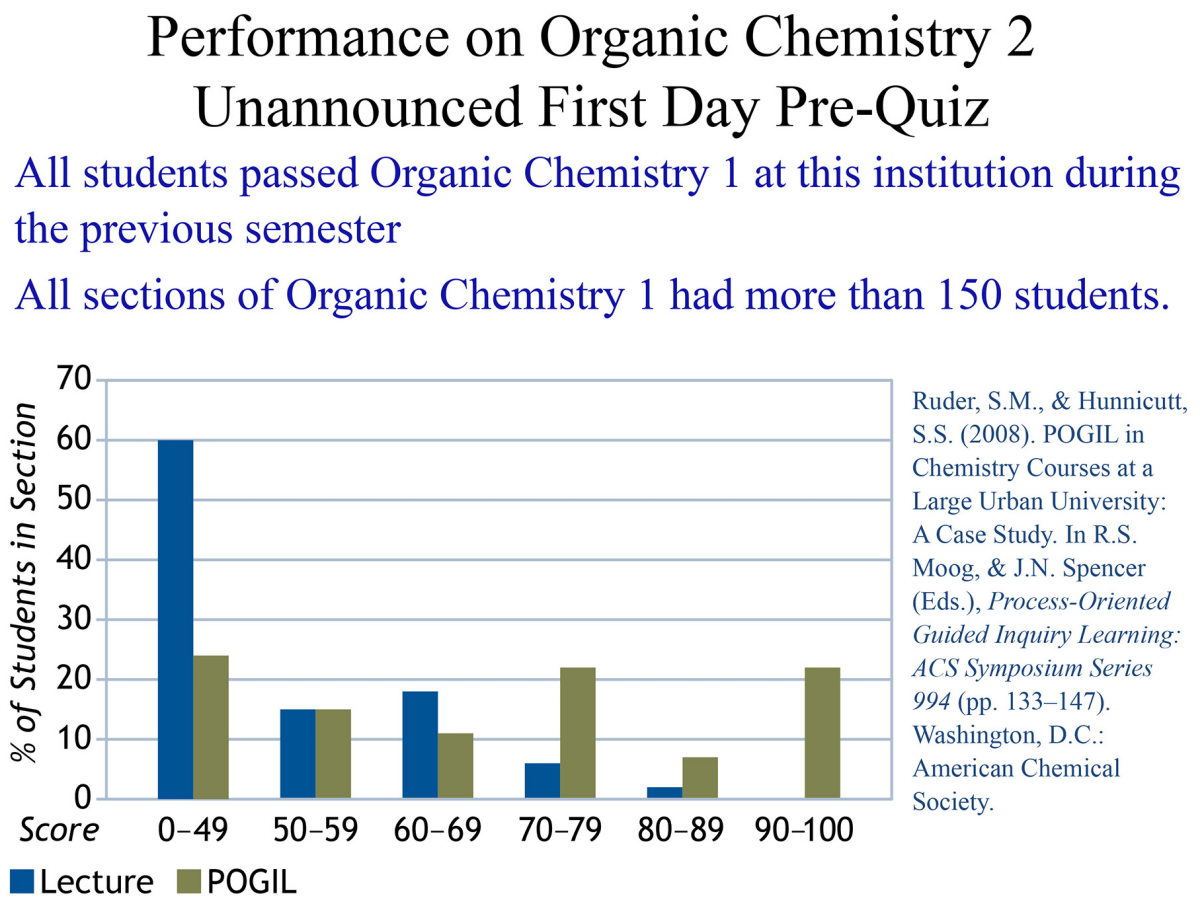
\includegraphics[width=0.50\linewidth]{pogil-prequiz.png}


\quest{10 min}


\Q How large were the classes at each of the universities shown above?

\begin{answer}[2em]
The left university had classes of about 24, and the right had over 150 students/section.
\end{answer}


\Q What are the measures of performance shown in each of the figures?

\begin{answer}[2em]
The left figure shows grade distributions, and the right figure shows pre-quiz scores.
\end{answer}


\Q What does the figure on the left suggest about POGIL's impact on student success?

\begin{answer}[6em]
\small
``Students in courses employing a POGIL instructional strategy achieved a significantly higher success rate (defined as receiving an A, B, or C in the course, as compared to a D, F or withdrawal) than students who had been taught by the same instructors in previous years using a more traditional lecture-oriented approach.
In both cases, the students were in classes of about 24 students each, and similar exams were used for both groups of students.'' (Moog 2014)
\end{answer}


\Q What does the figure on the right suggest about students' retention of knowledge?

\begin{answer}[6em]
\small
``A majority of the students (60\%) in the lecture section scored below 50 percent on the quiz, and none of the students achieved a score above 90 percent.
Less than five percent scored above 80 percent.
In contrast, fewer than a a quarter of the students from the POGIL section scored below 50 percent on this quiz, and about 30 percent of the students scored above 80 percent, with over one-fifth of the POGIL
students scoring above 90 percent.'' (Moog 2014)
\end{answer}

\newpage
\model{Common Methods}

Classes are often used to represent abstract data types, such as \java{Color} or \java{Point}.
They are also used to represent objects in the real world, such as \java{CreditCard} (see \ref{credit-card.tex}) or \java{Person}.

\begin{center}
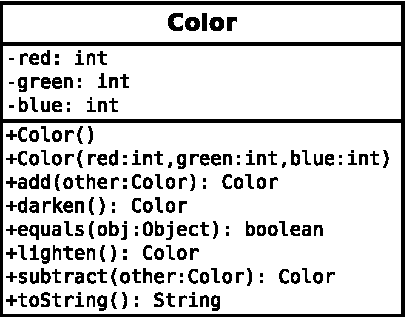
\includegraphics{Color.pdf}  % immutable
~~~~~
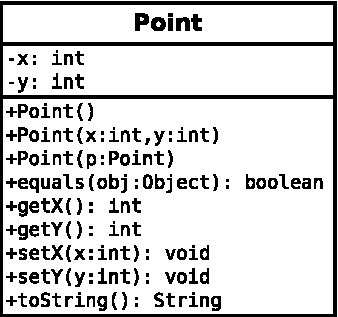
\includegraphics{Point.pdf}  % mutable
\end{center}

Classes generally include the following kinds of methods (in addition to others):
\begin{itemize}[itemsep=0pt]
\item \textbf{constructor} methods that initialize new objects
\item \textbf{accessor} methods (getters) that return attributes
\item \textbf{mutator} methods (setters) that modify attributes
\item \textbf{object} methods such as \java{equals} and \java{toString}
%\item \textbf{utility} methods which are generally static
\end{itemize}


\quest{20 min}


\Q Identify the constructors for the \java{Color} class.
What is the difference between them?
What arguments do they take?

\begin{answer}[3em]
There are two constructors: one that takes three integers for the RGB values, and other that takes a Color object. The latter is called a \emph{copy constructor}. Constructors do not return values.
\end{answer}


\Q What kind of constructor does the \java{Point} class have that the \java{Color} class does not?
What is the purpose of such a constructor?

\begin{answer}[3em]
The \java{Point} class also has a default constructor, which initializes attributes to their default value (most likely zero).
\end{answer}


\Q Identify an accessor method in the \java{Point} class.

\begin{enumerate}[itemsep=1pt]
\item Which instance variable does it get? \ans{{\tt this.x} or {\tt this.y}}
\item What arguments does the method take? \ans{none}
\item What does the method return? \ans{The value of \java{x} or \java{y}}
\end{enumerate}


\Q Identify a mutator method in the \java{Point} class.

\begin{enumerate}[itemsep=1pt]
\item Which instance variable does it set? \ans{{\tt this.x} or {\tt this.y}}
\item What arguments does the method take? \ans{The value of \java{x} or \java{y}}
\item What does the method return? \ans{nothing}
\end{enumerate}


\Q \label{immutable}
The \java{Color} class does not have accessors or mutators, but it provides methods that return lighter or darker \texttt{Color} objects.
Why do you think the class was designed this way?

\begin{answer}
Other than the constructor, there are no methods that change the \texttt{red}, \texttt{green}, and \texttt{blue} values.
This design makes the class immutable, which means that objects can be reused.
The \java{String} class is also designed this way.
\end{answer}


\vspace{2em}
\hrulefill

\vspace{1ex}
\textit{For the following questions, consider this portion of source code from the \java{Point} class.}
\vspace{1ex}

\begin{javalst}
    public Point() {
        this.x = 0;
        this.y = 0;
    }

    public boolean equals(Object obj) {
        if (obj instanceof Point) {
            Point p = (Point) obj;
            return this.x == p.x && this.y == p.y;
        }
        return false;
    }

    public String toString() {
        return String.format("(%d, %d)", this.x, this.y);
    }
\end{javalst}

%\hrulefill
%\vspace{1em}


\Q \label{expr}
What is the value of each expression below? (Don't just guess; read the source code above.)
\begin{javalst}
Point p1 = new Point();  Point p2 = new Point(0, 0);  Point p3 = new Point(3, 3);
\end{javalst}

\begin{multicols}{2}
\setlength{\defaultwidth}{5em}
\begin{enumerate}[itemsep=1pt]
\item \java{p1 == p1} \ans{true}
\item \java{p1.equals(p1)} \ans{true}
\item \java{p1 == p2} \ans{false}
\item \java{p1.equals(p2)} \ans{true}
\item \java{p1.equals(p3)} \ans{false}
\item \java{p2.toString()} \ans{"(0, 0)"}
\item \java{p2.equals("(3, 3)")} \ans{false}
\item \java{p3.equals("(3, 3)")} \ans{false}
\end{enumerate}
\end{multicols}


\Q What is the purpose of the \texttt{equals} and \texttt{toString} methods?

\begin{answer}[5em]
The \java{equals} method determines whether two objects have the same attribute values, and the \java{toString} method returns a \texttt{String} representation of the \texttt{Point} object.
These methods make it easier to work with user-defined data types.
\end{answer}


\Q What is the purpose of the \java{if}-statement in the \texttt{equals} method?

\begin{answer}
Since \java{equals} can take any type of \java{Object}, you need to check if the argument is a \java{Point} instance before using it as such.
\end{answer}


\Q How could you modify the \java{equals} method to cause both \ref{expr}d and \ref{expr}h to return \java{true}?

\begin{answer}[5em]
Change the last line to ~\texttt{return this.toString().equals(obj);}

You could instead add ~\texttt{if (obj instanceof String)}, but since the \texttt{String.equals} method takes an \texttt{Object}, there's no need to convert the \java{obj} parameter before calling \texttt{String.equals}.
\end{answer}

\vspace{2em}
\model{Credit Card}
% based on Model 2 of "Activity 10 - Class Design" by Helen Hu

Classes often represent objects in the real world.
In this section, you will design a new class that represents a \java{CreditCard} like the one below:

\begin{center}
% https://www.bankofamerica.com/credit-cards/

\includegraphics{credit-card.png}
\end{center}


\quest{15 min}


\Q Identify two or more attributes that would be necessary for the \java{CreditCard} class.
For each attribute, indicate what data type would be most appropriate.

\begin{answer}
Answers may include ~\verb|number:long|, ~\verb|expire:Date|, ~\verb|name:String|, ~\verb|code:int|, ~etc.
\end{answer}


\Q Using UML syntax, define two or more constructors for the \java{CreditCard} class.

\begin{answer}
\begin{javaans}
+CreditCard()
+CreditCard(number:long, name:String)
\end{javaans}
\end{answer}


\Q Define two or more accessor methods for the \java{CreditCard} class.
Include arguments and return values, using the same format as a UML diagram.

\begin{answer}[5em]
\begin{verbatim}
+getNumber(): long
+getExpire(): Date
+getName(): String
+getCode(): int
\end{verbatim}
\end{answer}


\Q Define two or more mutator methods for the \java{CreditCard} class.
Include arguments and return values, using the same format as a UML diagram.

\begin{answer}[5em]
\begin{verbatim}
+setNumber(number:long): void
+setExpire(expire:Date): void
+setName(name:String): void
+setCode(code:int): void
\end{verbatim}
\end{answer}


\Q Describe how you would implement the \java{equals} method of the \java{CreditCard} class.

\begin{answer}
Two credit cards would be considered equal if they have the same account number, assuming there are no duplicates in the bank.
\end{answer}


\Q Describe how you would implement the \java{toString} method of the \java{CreditCard} class.

\begin{answer}
The \java{toString} would print the account number, expiration date, and cardholder's name, each separated by a comma.
\end{answer}


\Q When constructing (or updating) a \java{CreditCard} object, which arguments would you need to validate?
What are the valid ranges of values for each attribute?

\begin{answer}[5em]
The number should have 16 digits, dates need to have valid months and days, names should be at most 22 letters and not contain digits or other characters, code should be 3--4 digits, etc.
\end{answer}


\end{document}
